Intuitively, an abstract state of the Parametric Hypercubes domain (\adomain) tracks disjunctive information relying on floating-point intervals of fixed width. A state of \adomain\ is made by a set of hypercubes of dimension $|\variables|$. Each hypercube has $|\variables|$ sides, one for each variable, and each side contains an abstract non-relational value for the corresponding variable. Each hypercube represents a set of admissible combinations of values for all variables. 

The name Hypercubes comes from the geometric interpretation of the elements of \adomain . The concrete state of a program with variables in $\variables$ is an environment in $\funzione{\variables}{\real}$. This can be isomorphically represented by a tuple of values where each item of the tuple represents a program variable. Seen in this way, the concrete state corresponds, geometrically, to \emph{a point} in the $|\variables|$-dimensional space. 
%Each dimension of the space represents the possible values that the corresponding variable of the program can assume. The concrete trace of a program is a sequence of points in such space (one for each state of the trace). 
The hypercubes of our domain \adomain\ are \emph{volumes} in the same $|\variables|$-dimensional space. 
%Each side of the hypercube is the concretization of the abstract value of the corresponding variable, and thus it corresponds to a set of values in that dimension of the space. The concretization of an hypercube is the set of all the points contained in its volume. A state in \adomain\ is composed by a set of hypercubes: its concretization is the union of all the volumes of its hypercubes.  In this way we track disjunctive information.

\vspace{-10pt}
\subsection{Lattice structure}
\vspace{-5pt}
An abstract state of \adomain\ tracks a \emph{set} of hypercubes, and each hypercube is represented by a tuple of abstract values. The dimension of these tuples is equal to the number of program variables.
%: this means that each variable is associated to a given item of the tuple (i.e., to a specific side of the hypercube). 
%Consider for instance a program in which $\variables = \{x_1, x_2\}$. In this case, the hypercubes of \adomain\ are 2D-rectangles. In particular, the two sides of a single hypercube are two abstract values, one for $x_1$ and one for $x_2$.
%A priori, our approach is modular w.r.t. the non-relational abstract domain we adopt to approximate the values of single variables inside an hypercube.
We abstract floating-point variables through intervals of real values. A set of hypercubes allows us to track disjunctive information, and this is useful when the values of a variable are clustered in different ranges.
%: instead of having a very big interval to cover them all (and which would cover also a lot of invalid values), we use two (or more) smaller intervals. Since it would be particularly expensive to perform all the lattice operators pointwisely, we partition the possible values into intervals of fixed width. As an example, suppose that the initial vertical velocity of the balls of our case study ranges between $50.0$ and $60.0$ or between $-60.0$ and $-50.0$. A single interval would approximate these values with $[-60.0 .. 60.0]$, while with our approach we track two intervals, $[-60.0 .. -50.0]$ and $[50.0 .. 60.0]$ (with fixed width $10.0$), which distinguish between balls thrown downwards and balls thrown upwards. 
The performance of this domain, though, becomes a crucial point, because the number of possible hypercubes in the space is potentially exponential with respect to the number of partitions along each spatial axis. 

First of all, the complexity is lightened by the use of a \emph{fixed} width for each variable, by partitioning the possible intervals, and by the efficiency of set operators on tuples. Then, another performance booster is the use of a smart representation for intervals: in order to store the specific interval range we just use a single integer representing it. This is possible because each variable $x_i$ is associated to an interval width (specific only for that variable), which we call $w_i$ and which is a parameter of the analysis. Each width $w_i$ represents the width of all the possible abstract intervals associated to $x_i$. More precisely, given a width $w_i$ and an integer index $m$, the interval uniquely associated to the variable $x_i$ is $[m \times w_i .. (m+1) \times w_i]$. Notice that the smaller the width associated to a variable, the more granular and precise the analysis on that variable (and the heavier computationally the analysis). In Section \ref{sec:semantics} we will show how to compute and adjust automatically the widths.

\textbf{Example:} Consider the case study of Section \ref{sec:case_study} and in particular the two variables \statement{px} and \statement{py}. Suppose that the widths associated to such variables are $w_1 = 10.0, w_2 = 25.0$. The hypercubes in this case are 2D-rectangles that can be represented on the Cartesian plane.
Each side of a hypercube is identified by an integer index, and a 2D hypercube is then uniquely identified by a pair of integers. For instance, the hypercube $h_1 = ( 0, 1 )$ represents $\statement{px} \in [0.0 .. 10.0]$ and $\statement{py} \in [25.0 .. 50.0]$, while the hypercube $h_2 = ( 0, 0 )$  associates $\statement{px}$ to $[0.0 .. 10.0]$ and $\statement{py}$ to $[0.0 .. 25.0]$. Figure \ref{fig:hcExample} depicts the two hypercubes associated to the initialization of the case study (i.e., $h_1$ and $h_2$). Instead, Figure \ref{fig:hcExample2} depicts the six hypercubes obtained after executing the first iteration of the \statement{while} loop.
%The ball is moving towards the right of the screen and is going downwards: this is coherent with the fact that the horizontal velocity is certainly positive (between $0.0$ and $60.0$), while the vertical velocity is certainly negative (between $-30.0$ and $-25.0$). 

\vspace{-10pt}
\begin{figure}
\centering
\subfloat[The abstract state after the initialization of the variables \statement{px,py}, when their widths are, respectively, $10.0$ and $25.0$]{
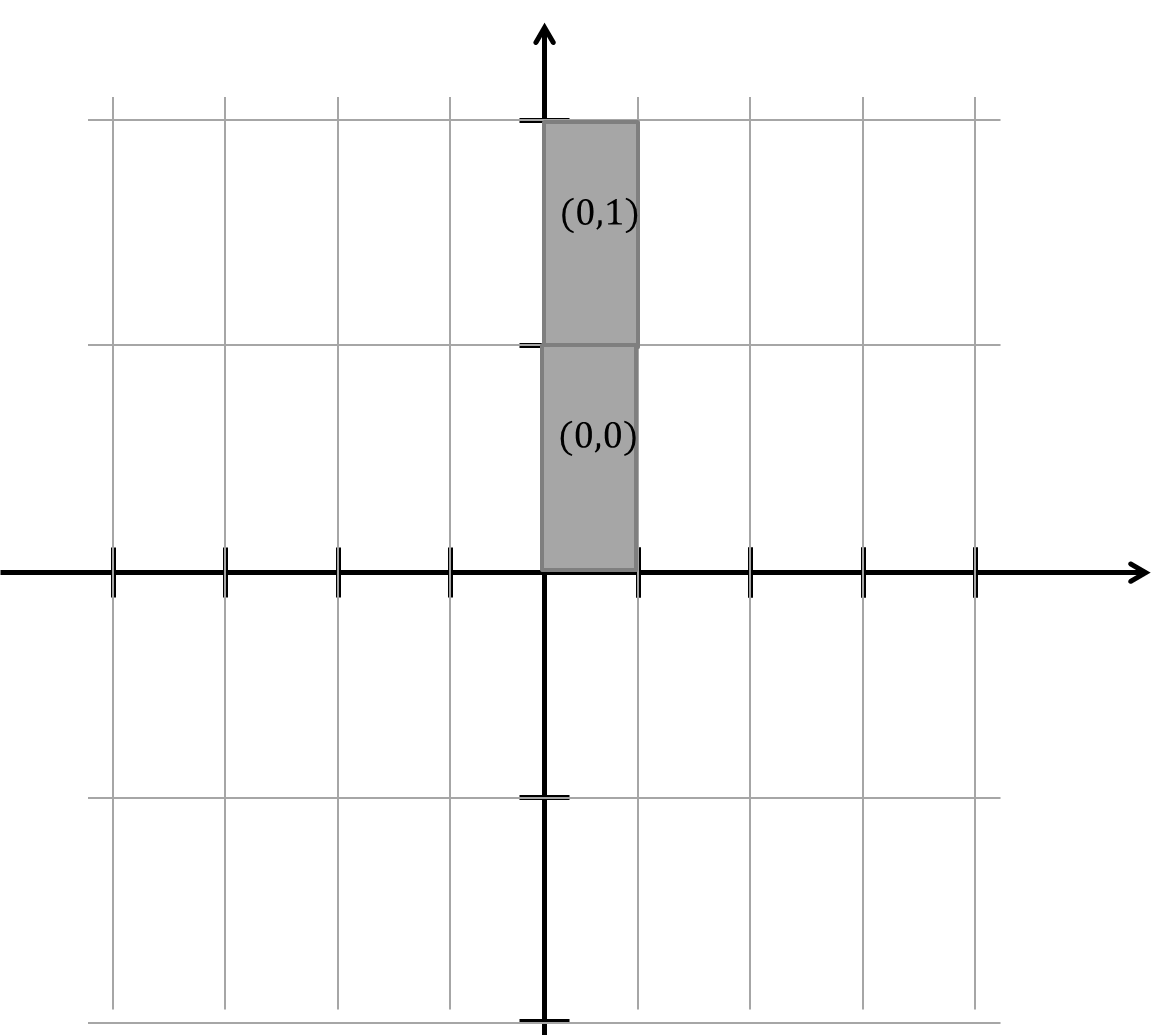
\includegraphics[scale=0.28]{Pics/example_hc_2d.png}
\label{fig:hcExample}
}\hspace{0.3cm}
\subfloat[The abstract state of \statement{px,py} after the first iteration of the loop (widths are, respectively, $10.0$ and $25.0$)]{
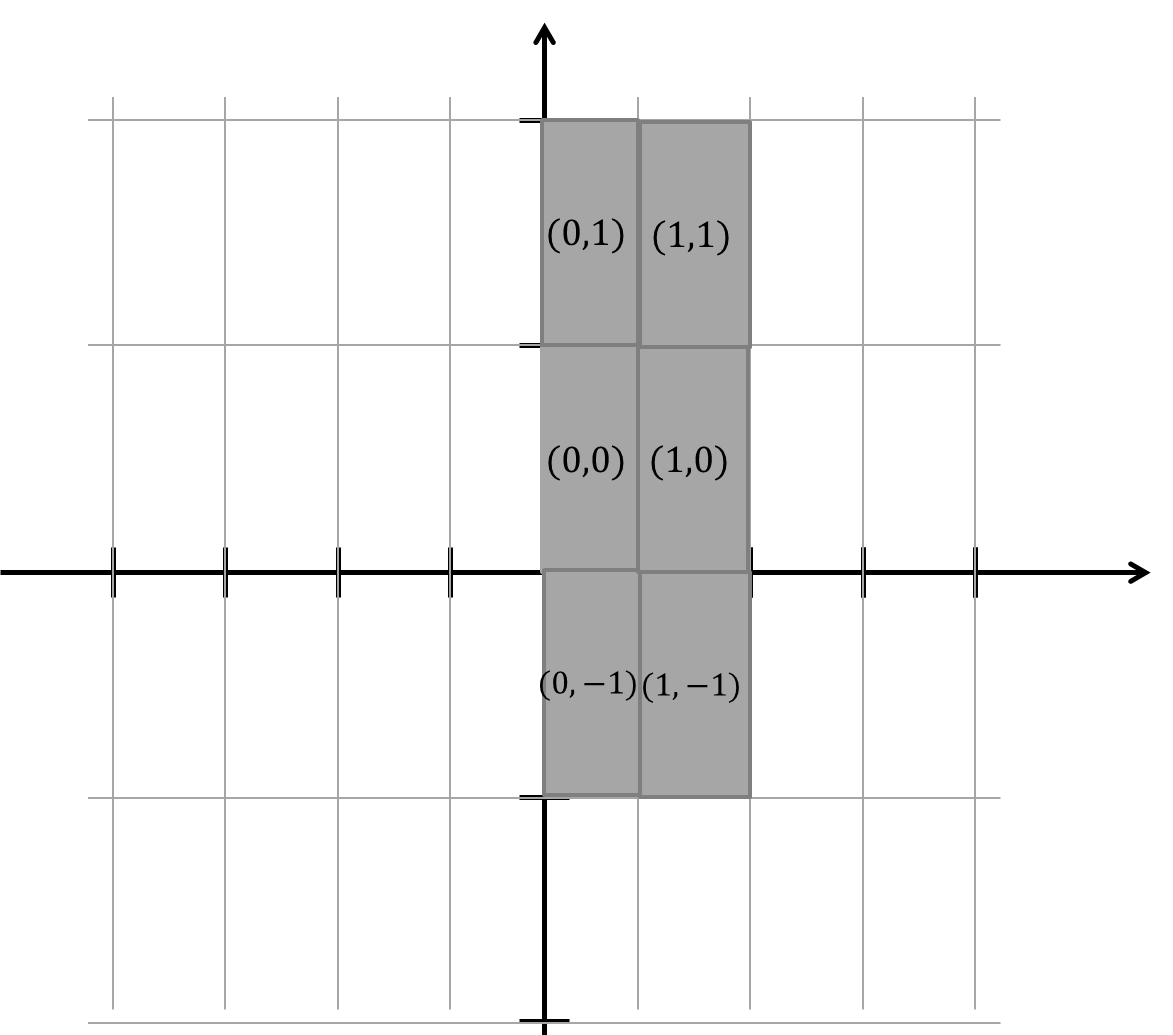
\includegraphics[scale=0.28]{Pics/example_hc_2d_2.png}
\label{fig:hcExample2}
}
\caption{Cartesian plans}
\end{figure}
\vspace{-10pt}


%\begin{figure}[ht]
%\begin{centering}
%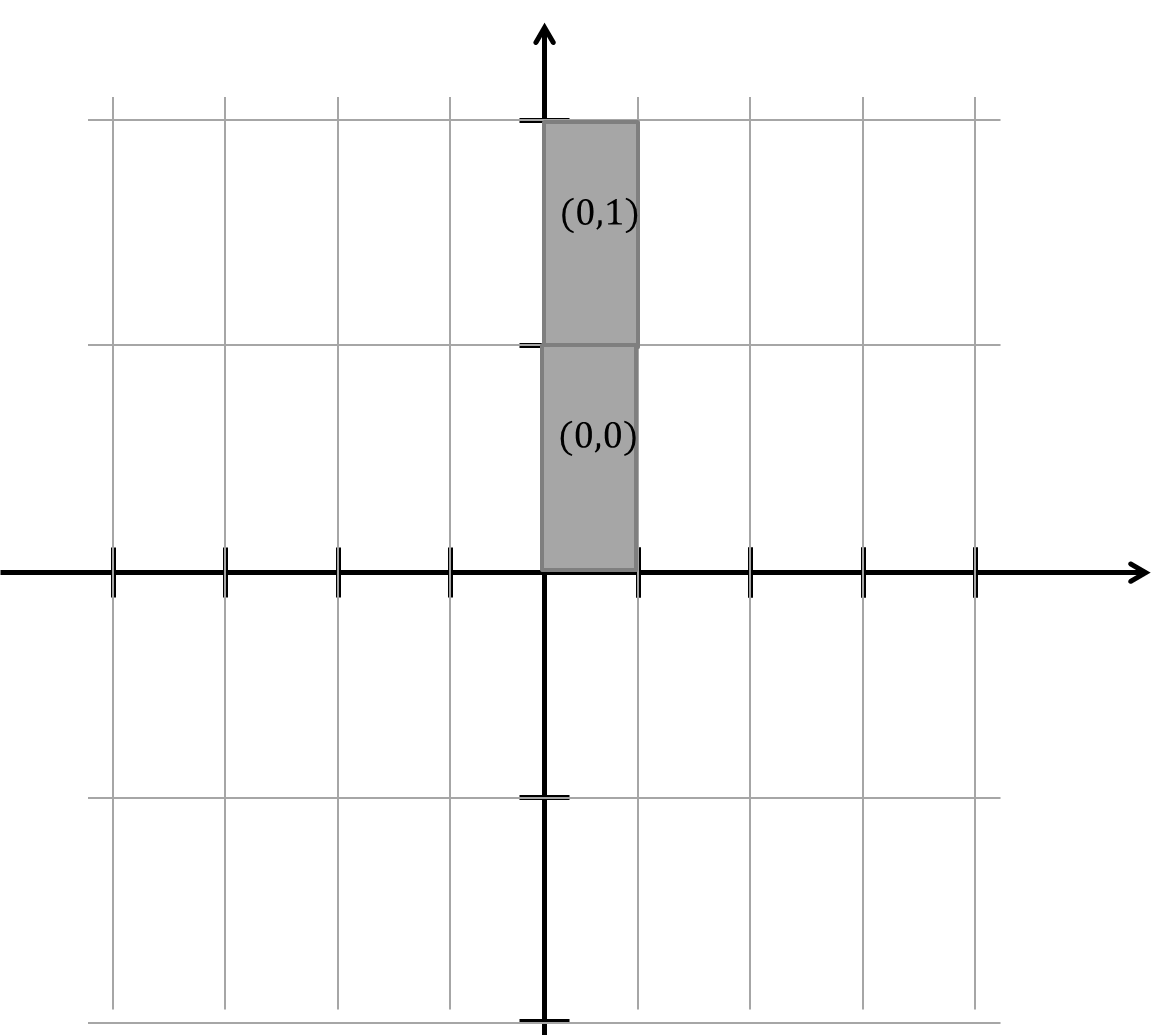
\includegraphics[scale=0.35]{Pics/example_hc_2d.png}
%\caption{The abstract state of the case study after the initialization of the variables (focusing the attention only on \statement{px,py}, when their widths are, respectively, $10.0$ and $25.0$)}
%\label{fig:hcExample}
%\end{centering}
%\end{figure}
%
%\begin{figure}[ht]
%\begin{centering}
%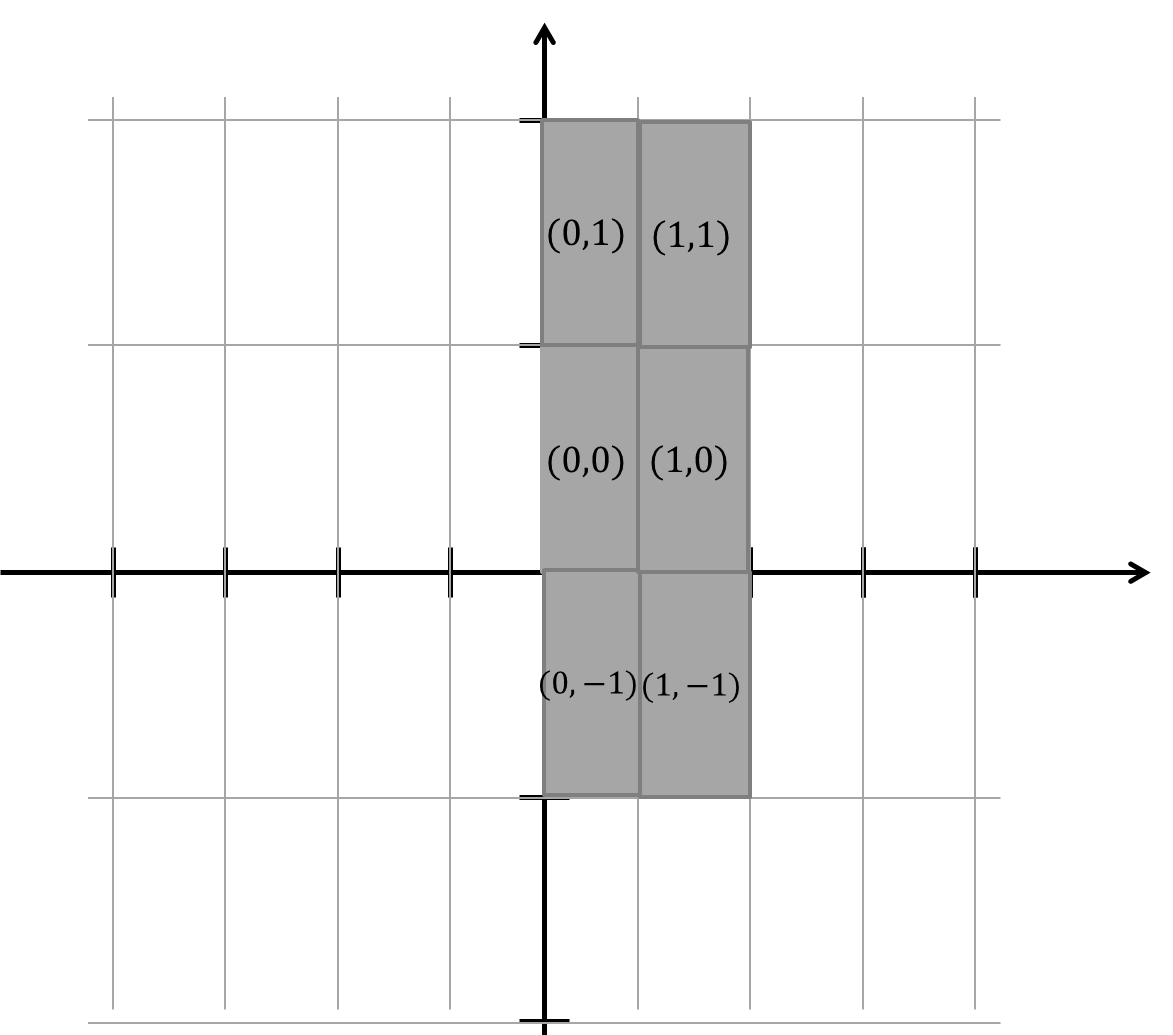
\includegraphics[scale=0.35]{Pics/example_hc_2d_2.png}
%\caption{The abstract state of the case study after the first iteration of the loop (focusing the attention only on \statement{px,py}, when their widths are, respectively, $10.0$ and $25.0$)}
%\label{fig:hcExample2}
%\end{centering}
%\end{figure}


We now formalize our abstract domain. Each abstract state is a set of hypercubes, where each hypercube is composed by $|\variables|$ integer numbers. The abstract domain is then defined by $\adomain = \wp(\integer^n)$ where $n = |\variables|$. The definition of lattice operators relies on set operators.
%: the partial order is defined through set inclusion, the lub and glb are set union and set intersection, respectively, while bottom and top are the empty set and the set containing all possible $n$-dimensional hypercubes, respectively. 
Formally, $\langle\wp(\integer^n), \subseteq, \cup, \cap, \emptyset, \integer^n\rangle$.

%\begin{lemma}
%$\langle\wp(\integer^n), \subseteq, \cup, \cap, \emptyset, \integer^n\rangle$ is a complete lattice.
%\begin{proof}
%The proof follows immediately by basic properties of set operators.
%\end{proof}
%\end{lemma}

\vspace{-10pt}
\subsection{Concretization function}
\vspace{-5pt}
We denote by $\agenericdomain$ the non-relational abstract domain on which our analysis is parameterized, and by $n$ the number of variables of the program. Let $\sigma \in \real^n$ be a tuple and $\sigma_i \in \real$ be the $i$-th element of such tuple. Also, let $\gamma_\agenericdomain : \funzione{\agenericdomain}{\wp(\real)}$ be the concretization function of abstract values of the non-relational abstract domain $\agenericdomain$, and $\function{getAbsValue}_v : \funzione{\naturals}{\agenericdomain}$ be the function that, given an integer index, returns the abstract value (in the domain $\agenericdomain$) which corresponds to that index inside the tuple $v$.
Then, the function $\gamma_{\aval} : \funzione{\wp(\agenericdomain^n)}{\wp(\real^n)}$ concretizes a set of hypercubes to a set of vectors of $n$ floating point values. Formally, $\gamma_{\aval}(\cel{V}) = \{\sigma : \exists v \in \cel{V} : \forall i \in [1..n] : \sigma_i \in \gamma_\agenericdomain(\function{getAbsValue}_v(i)) \}$ where $\cel{V} \in \wp(\agenericdomain^n)$ is a set of hypercubes.
Finally, based on $\gamma_{\aval}$, we can define the function $\gamma_{\adomain}$, which maps a subset $\cel{V}$ of $\wp(\agenericdomain^n)$ into an environment. The function $\gamma_{\adomain} : \funzione{\wp(\agenericdomain^n)}{\wp(\funzione{\variables}{\real})}$ concretizes the hypercubes domain. Formally, $\gamma_{\adomain}(\cel{V}) = \{[\statement{x} \mapsto \cel{\sigma}_{\avariableindex{\statement{x}}} : \statement{x} \in \variables] : \cel{\sigma} \in \gamma_{\aval}(\cel{V})\}$.  The function $\gamma_{\adomain}$ maps the vectors returned by $\gamma_{\aval}$ into concrete environments relying on the function $\avariableindexname : \funzione{\variables}{\naturals}$. The latter, given a variable, returns its index in the tuples which compose the elements of \adomain.

%Intuitively, we represent a concrete value as a tuple of real values (one for each variable of the program). The concretization of an abstract state $h \in \adomain$ is then a set of tuples. The concretization of $h$ is the union of all the concretizations of its hypercubes, i.e., all the points belonging to the volumes of its hypercubes. Each tuple of the concretization of $h$, then, is a point belonging to one hypercube of $h$. 

\vspace{-10pt}
\subsection{Convergence of the analysis}
\vspace{-5pt}
%The domain described so far does not ensure the convergence of the analysis. In fact, a \statement{while} loop may add new hypercubes with increased indices at each iteration, and the dimension of the abstract state (i.e., the hypercubes set) would increase at each iteration without converging. Thus, we need a way to force the convergence of the analysis. Given our abstract state representation, 
The number of hypercubes in an abstract state may increase indefinitely. In order to make the analysis convergent, we fix for each variable of the program a maximum integer index $n_i$ such that $n_i$ represents the interval $[n_i \times w_i .. +\infty]$. The same happens symmetrically for negative values. In this way, the set of indices of a given variable is finite, the resulting domain has finite height, and the analysis is convergent.

This approach may seem too rough since we establish the bounds of intervals before running the analysis. However, 
%this allows us to control the number of possible intervals in our hypercubes, and this is particularly important for the efficiency of the overall analysis. In addition, 
when analysing physics simulations we can use the initialization of variables and the property to verify in order to establish convenient bounds for the intervals. For instance, in the case study presented in Section \ref{sec:case_study} we are interested in checking if a ball stays in the screen, that is, if \statement{px} is greater than zero and less than a given value \statement{w} representing the width of the screen. Since we are only interested in proving that, once a ball has exited the screen, it does not come back, we can abstract together all the values that are greater than \statement{w}.

%Observe that more sophisticated widening operators could be used as an alternative to the adopted solution described above, but this could affect the performance of the resulting analysis.

%\subsection{Other data types or non-relational abstractions}
%\todogiulia{Secondo me questa subsection si puo' cancellare}
%As suggested before, for now we focus the application of our abstract domain to physics simulations, and for this reason we abstract floating point variables through intervals of fixed width. However, we may apply other kind of abstractions (e.g., the Sign domain) to our framework to consider other types of variables (integer, boolean, etc.). We will sketch other possible applications of our framework in Section \ref{sec:otherapplications}.

\vspace{-10pt}
\subsection{Offsets}
\vspace{-5pt}
A loss of precision may occur due to the fact that hypercubes proliferate too much, even using small widths. Consider, for example, the statement \statement{x = x + 0.01} (which is repeated at each iteration of the \statement{while} loop) with $1.0$ as the width associated to \statement{x}. If $[0.0 .. 1.0]$ was the initial interval associated to \statement{x}, the sequence of abstract states would be: $\{ [0.0 .. 1.0] \}$, $\{ [0.0 .. 1.0], [1.0 .. 2.0] \}$, $\{ [0.0 .. 1.0], [1.0 .. 2.0], [2.0 .. 3.0] \}$ and so on. At each iteration we would add one interval. 
%If the initial interval associated to \statement{x} was $[0.0 .. 1.0]$, after the first iteration we would obtain two intervals ($[0.0 .. 1.0]$ and $[1.0 .. 2.0]$) because the resulting interval would be $[0.01 .. 1.01]$, which spans over two fixed-width intervals. For the same reason, after the second iteration we would obtain three intervals ($[0.0 .. 1.0],[1.0 .. 2.0]$ and $[2.0 .. 3.0]$) and so on: at each iteration we add one interval. 

In order to overcome these situations, we further improve the definition of our domain: in each hypercube, each variable $v_i$ (associated to width $w_i$) is related to (other than an integer index $i$ representing the fixed-width interval $[i \times w_i .. (i+1) \times w_i]$) a specific offset $(o_m,o_M)$ \emph{inside} such interval. In this way, we use a sub-interval (of arbitrary width) inside the fixed-interval width, thereby restricting the possible values that the variable can assume. Both $o_m$ and $o_M$ must be smaller than $w_i$, greater than or equal to $0$ and $o_m \leq o_M$. Then, if $i$ and $(o_m,o_M)$ are associated to $v_i$, this means that the possible values of $v_i$ belong to the interval $[(i \times w_i) + o_m .. (i \times w_i) + o_M]$.

An element of our abstract domain is then stored as a map from hypercubes to tuples of offsets. In this way, we can keep the original definition of a hypercube as a tuple of integers, but we also map each hypercube to a tuple of offsets (one for each variable). Now an abstract state is defined by $M : \funzione{\integer^{|Vars|}}{{(\real \times \real)}^{|Vars|}}$, i.e., a map where the domain is the set of hypercubes, and the codomain is the set of tuples of offsets.

The least upper bound between two abstract states ($M=M_1 \sqcup M_2$) is then defined by $dom(M) = dom(M_1) \cup dom(M_2)$, and

$$
\forall h \in dom(M) : M(h) = \begin{cases}
M_1(h) & \mbox{if } h \in dom(M_1) \wedge h \notin dom(M_2) \\
M_2(h) & \mbox{if } h \in dom(M_2) \wedge h \notin dom(M_1) \\
merge(M_1(h),M_2(h)) & \mbox{otherwise }
\end{cases}$$
where $merge(o_1,o_2)$ creates a new tuple of offsets by merging the two tuples of offsets in input: for each pair of corresponding offsets (for example $(m_1,M_1)$ and $(m_2,M_2)$), the new offset is the widest combination possible (i.e., $(\min(m_1,m_2)$ and $\max(M_1,M_2))$). Note that this definition corresponds to the pointwise application of the least upper bound operator over intervals. The widening operator is extended in the same way: it applies the standard widening operators over intervals pointwisely to the elements of the vector representing the offsets.
